21. \begin{figure}[ht!]
\center{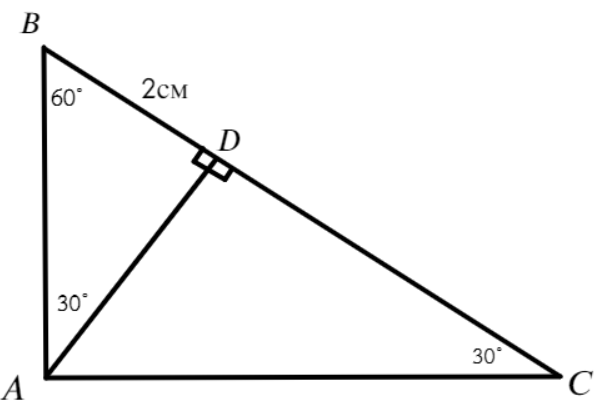
\includegraphics[scale=0.35]{g21.png}}
\end{figure}\\
$\angle BAD=\angle C=90^\circ-\angle B=90^\circ-60^\circ=30^\circ.$ В прямоугольном треугольнике $ABD$ катет $DB$ лежит напротив угла в $30^\circ,$ а значит гипотенуза $AB=2\cdot2=4$см. В прямоугольном треугольнике $ABC$ катет $AB$ лежит напротив угла в $30^\circ,$ значит гипотенуза $BC=2\cdot4=8$см. Таким образом, $DC=BC-DB=8-2=6$см.\\
